\documentclass[10pt,colorlinks=true,urlcolor=blue]{moderncv}
\usepackage{utopia}
\usepackage{breakurl}
\moderncvtheme[blue]{classic}
\usepackage[utf8]{inputenc}
%JLP\usepackage[resetlabels]{multibib}
\usepackage[backend=biber,defernumbers=true,refsection=section,sorting=ydnt,maxbibnames=999]{biblatex}
%\addbibresource{peer.bib}
%\addbibresource{pre.bib}
%\addbibresource{talks.bib}
%\addbibresource{other_talks.bib}
%\addbibresource{posters.bib}

%%
\addbibresource{pubs_peer_reviewed.bib}
\addbibresource{pubs_pre_prints.bib}
\addbibresource{pubs_conf.bib}
\addbibresource{pubs_other.bib}
\addbibresource{pubs_tech_reports.bib}
\addbibresource{pubs_excluded_entries.bib}
\addbibresource{talks_invited.bib}
\addbibresource{talks_other.bib}
%\addbibresource{talks_excluded_entries.bib}

\DeclareRefcontext{J}{labelprefix=J} %% Peer
\DeclareRefcontext{P}{labelprefix=P} %% Pre-prints
\DeclareRefcontext{I}{labelprefix=I} %% Invited Talks
\DeclareRefcontext{T}{labelprefix=T} %% Other Talks
\DeclareRefcontext{A}{labelprefix=A} %% Abstacts and Posters

\usepackage{pdfpages}

\usepackage{fancyhdr}
\pagestyle{fancy}
\pagenumbering{roman}
\chead{\textbf{Joshua T. Vogelstein Ph.D.}, Assistant Professor, JHU -- Curriculum Vitae}
\rhead{\thepage}


\usepackage[scale=0.8]{geometry}
\newcommand{\cvdoublecolumn}[2]{%
  \cvline{}{}{%
    \begin{minipage}[t]{\listdoubleitemmaincolumnwidth}#1\end{minipage}%
    \hfill%
    \begin{minipage}[t]{\listdoubleitemmaincolumnwidth}#2\end{minipage}%
    }%
}
%
% usage: \cvreference{name}{address line 1}{address line 2}{address line 3}{address line 4}{e-mail address}{phone number}
% Everything but the name is optxional
% If \addresssymbol, \emailsymbol or \phonesymbol are specified, they will be used.
% (Per default, \addresssymbol isn't specified, the other two are specified.)
% If you don't like the symbols, remove them from the following code, including the tilde ~ (space).

\newcommand{\cvreference}[7]{%
    \textbf{#1}\newline% Name
    \ifthenelse{\equal{#2}{}}{}{\addresssymbol~#2\newline}%
    \ifthenelse{\equal{#3}{}}{}{#3\newline}%
    \ifthenelse{\equal{#4}{}}{}{#4\newline}%
    \ifthenelse{\equal{#5}{}}{}{#5\newline}%
    \ifthenelse{\equal{#6}{}}{}{\emailsymbol~\texttt{#6}\newline}%
    \ifthenelse{\equal{#7}{}}{}{\phonesymbol~#7}}

  \AtBeginDocument{\recomputelengths}
  \firstname{Joshua T.~}
  \familyname{Vogelstein}
  % \address{Dept Biomedical Engineering \\
  % Institute for Computational Medicine \\
  %   Johns Hopkins University \\
  %   3400 N. Charles St., Clark Hall, Room 314 \\ }{Baltimore, MD
  %   21218}
  \email{jovo@jhu.edu}
  \homepage{jovo.me}

\begin{document}
\maketitle

I am currently an Assistant Professor of Biomedical Engineering in the Whiting School of Engineering at Johns Hopkins University, where I co-direct the \href{https://neurodata.io/}{NeuroData} lab, whose mission is to understand and improve animal and machine intelligences worldwide. As of September 2019, according to \href{https://scholar.google.com/citations?user=DWPfdT4AAAAJ&hl=en&oi=ao}{Google Scholar}, I have over 5,000 citations and an h-index of 29.  

\vspace{10pt}

Our website, \href{https://neurodata.io}{neurodata.io},  has the most up to date information regarding our team's
% 
% \begin{itemize}
	  \href{https://neurodata.io/publications/}{publications},
	  \href{https://neurodata.io/talks/}{talks},
	  \href{https://neurodata.io/presentations/#posters}{posters},
	  \href{https://neurodata.io/awards}{awards},
	  \href{https://neurodata.io/press}{press},
	  \href{https://github.com/jovo/cv/raw/master/CP_Vogelstein.pdf}{funding}, and
	  \href{https://blog.neurodata.io/}{blog}.
% \end{itemize}

\section{Education \& Training}

\cventry{08/12 -- 08/14}{Senior Research Scientist}{Dept's of Statistical Sciences \& Mathematics \& Neurobiology}{Supervised by Mauro Maggioni, Lawrence Carin, Guillermo Sapiro, and David Dunson}{Duke University}{\textbf{Research} Big data statistics, network statistics, graph matching.}

\cventry{01/11 -- 08/12}{Assistant Research Professor}{Department of Applied Mathematics and Statistics}{Supervised by Mauro Maggioni, Lawrence Carin, Jon Harer, and David Dunson}{Duke University}{\textbf{Research} Big data statistics, network statistics, graph matching.}

\cventry{12/09 -- 01/11}{Post-Doctoral Fellow}{Department of
  Applied Mathematics and Statistics}{Supervised by Carey E.~Priebe}{Johns Hopkins University}{\textbf{Research} Statistics of populations of networks.}

  \cventry{2003 -- 2009}{Ph.D in Neuroscience}{\newline Johns Hopkins School of Medicine, Supervised by Eric Young}{\newline \textbf{Dissertation} OOPSI: a family of optical spike inference algorithms for inferring neural connectivity from population calcium imaging
}{}{}

\cventry{2009 -- 2009}{M.S. in Applied Mathematics \& Statistics}{ Johns Hopkins University}{}{}{}

\cventry{1998 -- 2002}{B.A. in Biomedical Engineering}{Washington University, St.~Louis}{}{}{}


\subsection{Summer Workshops}

\cventry{06/08 -- 07/08}{Molecular Biology Summer Workshop}{Smith College, Mass, USA}{}{}{}

\cventry{07/08 -- 07/08}{Advanced Techniques in Molecular Neuroscience}{Cold Spring Harbor, New York, USA}{}{}{}

\cventry{06/05 -- 07/05}{Imaging Structure and Function of the Nervous System (audited)}{Cold Spring Harbor, New York, USA}{}{}{}

\cventry{06/04 -- 07/04}{Advanced Course in Computational Neuroscience}{Obidos, Portugal}{}{}{}



\section{Positions  Held}

\subsection{Current Academic Positions}
\cventry{08/14 -- now}{Assistant Professor}{Department of Biomedical Engineering}{Johns Hopkins University (JHU)}{}{}
\cventry{08/14 -- now}{Core Faculty}
{Institute for Computational Medicine  (ICM)}{}{}{}
\cventry{08/14 -- now}{Core Faculty}
{Center for Imaging Science (CIS)}{}{}{}
\cventry{08/15 -- now}{Steering Committee}
{Kavli Neuroscience Discovery Institute (KNDI)}{}{}{}

\subsection{Current Joint Appointments, Affiliations, and Activities}

\cventry{09/19 -- now}{Joint Appointment}{Department of Biostatistics}{Johns Hopkins University (JHU)}{}{}
\cventry{08/15 -- now}{Joint Appointment}{Department of Applied Mathematics and Statistics}{}{}{}
\cventry{08/14 -- now}{Joint Appointment}{Department of Neuroscience}{}{}{}
\cventry{08/14 -- now}{Joint Appointment}{Department of Computer Science}{}{}{}
\cventry{08/14 -- now}{Assistant Research Faculty}{Human Language Technology Center of Excellence}{}{}{}
\cventry{10/12 -- now}{Affiliated Faculty}{Institute for Data Intensive Engineering and Sciences}{}{}{}


\cventry{08/18 -- now}{\href{https://www.bme.jhu.edu/graduate/mse/degree-requirements/biomedical-data-science/}{Director of Biomedical Data Science Focus Area}}{}{}{}{}
\cventry{05/16 -- now}{Visiting Scientist}
{Howard Hughes Medical Institute}{Janelia Research Campus}{}{}
\cventry{01/11 -- now}{Co-Founder \& Co-Director}{\href{http://neurodata.io}{NeuroData} (formerly Open Connectome Project)}{}{}{}




\subsection{Previous  Positions \& Affiliations}
% \subsection{Academic}

\cventry{08/15 -- 07/18}{Co-Developer}{Computational Medicine Minor}{}{}{\url{http://icm.jhu.edu/academics/undergraduate-minor/}}
\cventry{08/14 -- 08/18}{\href{http://icm.jhu.edu/academics/undergraduate-minor/}{Director of Undergraduate Studies}}{Institute for Computational Medicine}{}{}{}
\cventry{05/15 -- 07/17}{Co-Founder and Faculty Advisor}{\href{http://medhacks.org}{MedHacks}}{}{}{}
\cventry{10/12 -- 08/14}{Endeavor Scientist}{Child Mind Institute}{}{}{}
\cventry{08/12 -- 08/14}{Affiliated Faculty}{Kenan Institute for Ethics}{}{}{Duke University}
\cventry{08/12 -- 08/14}{Adjunct Faculty}{Department of Computer Science}{}{}{}
\cventry{07/04 -- 07/12}{Chief Data Scientist}{Global Domain Partners, LLC}{}{}{}
\cventry{06/01 -- 09/01}{Research Assistant}{Prof. Randy O'Reilly, Dept.~of Psychology}{}{}{University of Colorado}
\cventry{06/00 -- 09/00}{Clinical Engineer}{Johns Hopkins Hospital}{}{}{}
\cventry{06/99 -- 08/99}{Research Assistant under Dr. Jeffrey Williams}{Dept. of Neurosurgery, Johns Hopkins Hospital}{}{}{}
\cventry{06/98 -- 08/98}{Research Assistant under Professor Kathy Cho}{Dept. of Pathology, Johns Hopkins School of Medicine}{}{}{}



\section{Entrepreneurial Activities}

\subsection{Founding Companies}

\cventry{01/17 -- now}{Co-Founder}{\href{http://gigantum.io}{gigantum}}{}{}{}
\cventry{01/16 -- now}{Co-Founder}{\href{http://www.d8alab.com}{d8alab}}{}{}{}

\subsection{Advisory Board}

\cventry{10/18 -- now}{Advisory Board}{\href{https://mind-x.io/}{Mind-X}}{}{}{}
\cventry{01/17 -- now}{Advisory Board}{\href{https://www.pivotalpath.com/}{PivotalPath}}{}{}{}

\subsection{Ad Hoc Consulting}

\cventry{2017}{Consultant}{\href{https://www.greenspringassociates.com}{Greenspring Associates}}{}{}{}

\cventry{2016}{Consultant}{Scanadu}{}{}{}




\section{\href{https://neurodata.io/about/awards/}{Awards \& Honors}}

%\cventry{2017}{\href{http://www.hpdc.org/2017/awards/best-paper-award}{Best Presentation Award HPDC}}{Mhembere et al. (2017)}{}{}{}
%\cventry{2017}{Nonparametric Statistics of the American Statistical Association Student Paper Award}{Lee et al. (2017)}{}{}{}
\cventry{2014}{F1000 Prime Recommended}{Vogelstein et al. (2014)}{}{}{}
\cventry{2013}{Spotlight}{Neural Information Processing Systems (NIPS)}{}{}{}
\cventry{2011}{Trainee Abstract Award}{Organization for Human Brain Mapping}{}{}{}
\cventry{2008}{Spotlight}{Computational and Systems Neuroscience (CoSyNe)}{}{}{}
\cventry{2002}{Dean's List}{Washington University}{}{}{}


%\section{Publications}
%\begin{refsection}[peer.bib]
\begin{refsection}[pubs_peer_reviewed.bib] 
\newrefcontext{J}
\nocite{*}
\defbibnote{a1}{\textbf{(52 articles published/accepted; top 10 cited 2,944 times; H-index 29)}}
\printbibliography[%
    title=\href{https://neurodata.io/publications/\#peer_reviewed}{Peer-Reviewed Journal Publications},%
    prenote=a1,% 
    heading=bibliography%
    ]
\end{refsection}



%\section{\href{https://neurodata.io/publications/\#pre_prints}{Pre-Prints}}
\begin{refsection}[pubs_pre_prints.bib] %, pubs_excluded_entries.bib]
\newrefcontext{P}
\nocite{*}
\printbibliography[%
    title=\href{https://neurodata.io/publications/\#pre_prints}{Pre-Prints},%
    heading=bibliography%
    ]
\end{refsection}



%\section{\href{https://neurodata.io/talks/}{Invited Talks}}
\begin{refsection}[talks_invited.bib]
\newrefcontext{I}
\nocite{*}
\printbibliography[%
    title=\href{https://neurodata.io/talks/}{Invited Talks},%
    heading=bibliography%
    ]
\end{refsection}



%\section{\href{https://neurodata.io/talks/}{Other Talks}}
\begin{refsection}[talks_other.bib, talks_excluded_entries.bib]
\newrefcontext{T}
\nocite{*}
\printbibliography[%
    title=\href{https://neurodata.io/talks/}{Other Talks},%
    heading=bibliography%
    ]
\end{refsection}



%\section{\href{https://neurodata.io/posters/}{Abstracts \& Posters}}
\begin{refsection}[pubs_conf.bib]
\newrefcontext{A}
\nocite{*}
\printbibliography[%
    title=\href{https://neurodata.io/posters/}{Abstracts \& Posters},%
    heading=bibliography,%
    ]
\end{refsection}




%%% Current Funding
\section{\href{https://neurodata.io/about/funding/}{Funding}}

\subsection{Current Funding}

% todo uli grant

\cventry{9/19 -- 8/22}{
    {Accessible technologies for high-throughput, whole-brain reconstructions of molecularly characterized mammalian neurons}}%
    {NIH}%
    {For a complete understanding of how the brain works, there is a
        need for a comprehensive parts list (all of the cells in the
        brain) along with knowledge of how those parts are connected.
        Current molecular technology has advanced the inventory of cell
        types in the brain, but detailed information about the circuits
        they form is limited. Dr. Mueller’s group will develop scalable
        and affordable cellular imaging and neuro-informatics tools,
        running preliminary experiments to connect the transcriptome to
        anatomy, in mice. Tools will be made available to researchers,
        to help accelerate the creation of detailed maps at cell
        resolution showing circuitry in whole brains.}
    {\$938,433}
    {Mueller (PI)}{}

    \cventry{12/19 -- 11/23}{
    {Understanding and improving robust learning against adversarial attacks}}%
    {DARPA GARD}%
    { The overall goal of the proposal is to develop technologies for the brain wide reconstruction of axonal arbors of molecularly defined neurons. The proposal aims at overcoming barriers in neuronal labeling, imaging and computation to achieve this goal, and to develop a technology platform that can be scaled to all neurons of the brain.}
    {}
    {Arora (PI)}{}

\cventry{12/19 -- 11/23}{
    {Brain Networks in Mouse Models of Aging}}%
    {NIH}%
    {
        There is a rapid growth in the number of people living with
        Alzheimer's disease, and only 25\% get diagnosed; still we do
        not know its etiology or have effective treatments. To examine
        factors which contribute to switching from normal to
        pathological aging we focus on the APOE polymorphic alleles. The
        causes for increased risk, or conversely resilience, conferred
        by the major APOE alleles are not known. The APOE4/4 genotype is
        the main genetic risk for late onset Alzheimer's disease (AD),
        and is associated with a 30-55\% risk of developing mild
        cognitive impairment or AD by age 85, compared to 10-15\% for
        the APOE3/3 genotype. In contrast APOE2 is under-represented in
        AD patients, and it has been associated with longevity. To help
        understand the mechanisms through which APOE genes and their
        products differentially modulate the brain and its circuits to
        switch from healthy to pathological aging, we will take an
        integrative and unbiased multi-disciplinary approach using
        homozygous targeted replacement APOE2, APOE3, and APOE4 mice
        expressing the major human APOE isoforms, under the control of
        the mouse endogenous ApoE promoter. APOE2 mice have a
        significantly longer lifespan than APOE3 mice, which in turn
        have a significantly longer lifespan than APOE4 mice. These mice
        reasonably match the human APOE-genotype/lifespan data. To model
        the human immune response to aging we will use double-transgenic
        mice that express human NOS2 gene products. This modification
        enables nitric oxide (NO) production and immune activity
        regulated by NO to better mimic the human response. Our models
        include male and female APOE2/HN (APOE2/2 + human NOS2 on a
        mouse Nos2-/- background), APOE3/HN, and APOE4/HN mice, at 2
        ages corresponding to middle and old human age.  Mice will be
        characterized with a cognitive behavioral battery, and with MRI
        to determine selective vulnerability of brain networks. Our
        imaging measures will be based on volume, vascular perfusion,
        and diffusion tensor imaging; and will provide connectomes and
        network measures. RNA-Seq transcriptomics will identify
        differential expression of gene products associated with APOE
        genotypes, during aging. We will use an unbiased statistical
        approach to map molecular pathways underlying the behavioral and
        imaging phenotypes for aging.  Our efforts will help build
        models that explain the influence of APOE genotypes on age and
        AD associated network vulnerability. We expect to hone in on
        pathways involved in aging, AD, inflammation, and oxidative
        phosphorylation. To test models, we will add a stressor
        conferring risk in aging and AD, through a high fat/high sugar
        diet (mimicking the Western diet). We will assess behavioral,
        and MRI phenotypes, in conjunction with transcriptomics, and
        determine through pathway analysis how diet shifts the predicted
        outcomes in male and female APOE2/HN, APOE3/HN and APOE4/HN
        mice.  Our research will reveal mechanisms through which APOE
        interacts with environmental stressors to confer vulnerability,
        or resilience to select brain circuits during aging 
    }
    {\$205,998}
    {Badea (PI)}{}

        
\cventry{7/19 -- 6/24}{
    {Reproducible imaging- based brain growth charts for psychiatry}}%
    {NSF}%
    {
    Major psychiatric illnesses are increasingly understood as disorders of brain development, which has led to large-scale studies of youth that combine multi-modal neuroimaging with clinical phenotyping. Together, such data have emphasized the promise of objective ?growth charts? of brain development.  However, synergies across major efforts remains unrealized due to use of different clinical instruments, different scanning protocols, challenges in informatics, and difficulties in data integration. In this proposal, we will overcome these obstacles by leveraging advances in multivariate harmonization and analysis techniques to build highly reproducible growth charts of human brain development. To do this, we will aggregate and harmonize eight existing large-scale developmental imaging studies, comprising over 10,000 participants between the age of 5- 24 (Aim 1). We will use this harmonized data to build generalizable indices of normal network brain development (Aim 2). Finally, developmental abnormalities within specific brain networks will be linked to dimensions of psychopathology (Aim 3). Critically, all code, data, and derived indices will be shared publicly, creating a massive new resource to accelerate research in the developmental neuroscience community (Aim 4). In sum, this proposal will have provide a new data resource, yield reproducible growth charts of brain development, and delineate novel mechanisms regarding the developmental basis of psychopathology in youth
    }
    {\$73,570}
    {Satterthwaite (PI)}{}


\cventry{5/17 -- 4/20}{
    \href{http://grantome.com/grant/NSF/DMS-1921310}%
    {Multiscale Generalized Correlation: A Unified Distance-Based Correlation Measure for Dependence Discovery}}%
    {NSF}%
    {This project aims to establish a unified methodology framework for statistical testing in highdimensional, noisy, big data, through theoretical advancements, comprehensive simulations, and real data experiments}%
    {\$200,000}%{This work was partially supported by the National Science Foundation award DMS1712947}%
    {Shen (PI) 1712947}{}


\cventry{7/17 -- 6/20}{
   \href{http://grantome.com/grant/NIH/R01-DC016784-02}%
   {CRCNS US-German Res Prop: functional computational anatomy of the auditory cortex}}%
    {NIH}%
    {The goal of this project is to create a robust computational framework for analyzing the cortical ribbon in a specific region: the auditory cortex}%
    {\$747,143}
    {Ratnanather (PI) 1R01DC016784-01}{}


\cventry{10/16 -- 9/20}%
    {What Would Tukey Do?}%
    {DARPA D3M}%
    {The goal is to develop theory \& methods for generating a discoverable archive of data modeling primitives and for automatically selecting model primitives and for composing selected primitives into complex modeling pipelines based on user-specified data and outcome(s) of interest}%
    {\$4,406,360}%
    {Priebe (PI) FA8750-17-2-0112}{}


\cventry{9/17 -- 8/22}{
   \href{http://grantome.com/grant/NIH/U19-NS104653-02}%
    {Sensorimotor processing, decision-making, and internal states: towards a realistic multiscale circuit model of the larval zebrafish brain}}%
    {NIH U19}%
    {The general goal of the proposal is to generate a realistic multiscale circuit model of the larval zebrafish’s brain – the multiscale virtual fish (MSVF). The model will span spatial ranges from the nanoscale at the synaptic level, to local microcircuits to inter-area connectivity - and its ultimate purpose is to explain and simulate the quantitative and qualitative nature of behavioral output across various timescales}%
    {\$210,000}%
    {Engert (PI) 1U19NS104653-01}{}


\cventry{1/18 -- 12/19}{
    {Connectome Coding at the Synaptic Scale}}%
    {Schmidt Sciences}%
    {This project will study learning and plasticity at an unprecedented scale, revealing the dynamics of large populations of synapses comprising an entire local cortical circuit. No previously conducted experiment could answer the questions about the dynamics of large populations of synapses, which is crucial to understanding the learning process}%
    {\$125,000}%
    {Vogelstein (PI)}{}


\cventry{11/17 -- 10/21}{
    {Lifelong Learning Forests}}%
    {DARPA L2M}%
    {Our Lifelong Learning Forests (L2Fs) will learn continuously, selectively adapting to new environments and circumstances utilizing top-down feedback to impact low-level processing, with provable statistical guarantees, while maintaining computational tractability at scale.  }%
    {\$8,000,000}%
    {Vogelstein (PI)}{}


\cventry{11/17 -- 10/21}{
    {Continual Learning Across Synapses, Circuits, and Brain Areas}}%
    {DARPA L2M}%
    {Our primary goal will be to develop the pre-processing analysis pipeline for the imaging data collected in this project}%
    {\$19,940}%
    {Tolias (PI)}{}


\cventry{7/18 -- 6/21}{
   \href{http://grantome.com/grant/NSF/MCB-1807546}%
    {SemiSynBio: Collaborative Research: YeastOns: Neural Networks Implemented in Communication Yeast Cells}}%
    {NSF}%
    {The goal is to provide neuroscience and machine learning expertise to guide the design of the computational learning capabilities of the system}%
    {\$599,757}%
    {Shulman (PI)}{}

\cventry{7/17 -- 6/20}{
    \href{https://www.nsf.gov/awardsearch/showAward?AWD_ID=1707298}%
    {NeuroNex Innovation Award: Towards Automatic Analysis of Multi-Terabyte Cleared Brains}}%
    {NSF, 16-569 Neural System Cluster}%
    {Three complimentary changes are revolutionizing the way neuroscientists study the brain. First, experimental advances allow neurobiologists to ``clear'' brains so that they become transparent, with the exception of a set of neurons that can be selected on the basis of their location, response properties, and genetic make-up. Second, technological advances have resulted in microscopes that can simultaneously image an entire ``sheet'' of this brain, thereby enabling rapid acquisition of whole brain volumes. Third, researchers are taking steps to educate neuroscientists to acquire these data. Together, this will result in a massive upswing in adoption of this experimental modality. However, acquiring the data is one step in the upward spiral of science that will yield transformative scientific results. The subsequent steps are computational. This project will develop cyberinfrastructure resources and software that enable storage and access of large CLARITY brain imaging datasets, alignment and registration to reference anatomical atlas and visualization of the datasets. Additional capabilities for automatic identification and localization of cell bodies and statistical analysis will be provided. The PIs will run annual hackathons for college students and sponsor a summer internship program for undergraduates to broaden the educational efforts in software development for neuroscience. Finally, mobile compliant digital education content will be created to complement existing online courses to target STEM students, and educate global citizens.
%
This project will build a prototype pipeline that operates on raw CLARITY brains and outputs the statistics of locations of cells in each region in the Allen Reference Atlas, as well as estimates of connectivity and similarity across regions and conditioned on different contexts. To do so, the PIs will leverage modern mathematical statistics (such as Large Deformation Diffeomorphic Metric Mapping for registration, Deep Learning and Random Forests for segmentation, and Statistical Graph Theory for analysis of the resulting conenctomes), as well as modern computational tools, including Docker containers to facilitate full reproducability, and semi-external memory algorithms and cloud computing to enable scalable analytics. To reach out to the broader community and educate them in the use of these tools, this project will provide tutorials deployed in the cloud. Together, this will facilitate the large community of users to both collect and analyze their data with ease. Many of the tools developed as part of this project will be easily extensible to other experimental modalities and neuroscience communities
    }
    {\$800,000}{Vogelstein (PI) 1707298}{}

\subsection{Past Funding}
% \subsection{Link to \href{https://github.com/jovo/cv/raw/master/CP_Vogelstein.pdf}{Current \& Pending}}
% \subsection{Past Funding}

\cventry{10/17 -- 9/18}{
    Brain Ark}
    {Dog Star Technologies}
    {}
    {Vogelstein (PI), 90074647}
    {}

\cventry{1/17 -- 10/18}{
    \href{https://nsf.gov/awardsearch/showAward?AWD_ID=1649880&HistoricalAwards=false}%    
    {Brain Comp Infra: EAGER: BrainLab CI: 
        Collaborative, Community Experiments with Data-Quality 
        Controls through Continuous Integration}}
    {NSF}
    {
    The brain research community needs to increase the practice of sharing and combining data sets to increase the power of statistical analyses and to gain the most knowledge from collected data. This project aims to build a prototype system called BrainLab CI that will facilitate meaningful integration of thousands of publicly available Magnetic Resonance Imaging (MRI) and neurophysiology data sets, and allow researchers to define and conduct new large-scale community-level experiments on these data. BrainLab CI has the potential to transform research practice in neuroscience by overcoming major obstacles to data sharing: Scientists will be able to share data without losing control over data quality, and will maintain full visibility into how all subsequent experiments use their data and algorithms. This project may consequently drive a change in scientific culture by encouraging data sharing and the development of common analysis tools, and resulting accelerated discovery from connecting ideas, tools, data, and people. This project therefore aligns with the NSF mission to promote the progress of science and to advance the national health, prosperity and welfare.
%
The BrainLab CI prototype system will provide new paradigms for combining different analytic methods, meta-analysis with raw data, comparing the results of different laboratories and even synthesizing new experiments by combining different studies. An experimental-management software system will be deployed that allows users to construct community-wide experiments that implement data and metadata controls on the inclusion and exclusion of data. Example of controls include: requiring specific metadata, that data are registered to a given atlas, or that data are collected using specific experimentation protocols. BrainLab CI will initially focus on two different experimental patterns: (1) An incremental experiment defines an experiment against an existing data set which then opens to additional community contributions of data; and (2) a derived experiment forks/branches an existing experiment, allowing a researcher to change properties, such as an acceptance criteria or analysis algorithm, but otherwise run the same pipeline against the same inputs. The system will allow each experiment to maintain online dashboards showing how additional data changes results with complete provenance. To develop and validate the BrainLab CI prototype, several community experiments will be developed for MRI and for neurophysiology (including both optical and electrical physiology) data. These research domains were chosen because of the great potential gains for increased sharing of laboratory data in these domains.
%
This Early-concept Grants for Exploratory Research (EAGER) award by the
CISE Division of Advanced Cyberinfrastructure is jointly supported by
the SBE Division of Behavioral and Cognitive Sciences, with funds
associated with the NSF Understanding the Brain activity including for
developing national research infrastructure for neuroscience, and
alignment with NSF objectives under the National Strategic Computing
Initiative%
    }
    {Burns (PI), ACI-1649880}{}

\cventry{5/15 -- 8/18}{
    From RAGs to Riches: Utilizing Richly Attributed Graphs to Reason from Heterogenous Data}
    {DARPA}
    {}
    {Vogelstein (PI), N66001-15-C-4041}{}

\cventry{9/14 -- 6/19}{
    \href{http://grantome.com/grant/NIH/R01-NS092474-01}%    
    {Synaptomes of Mouse and Man}}
    {NIH}
    {
    The synapse is the principle active signaling component of the brain's neuronal circuitry. Synapses are highly complex, plastic, strongly modulated and deeply diverse entities, and their molecular complexity and diversity are fundamental to all synaptic circuit development and function. Moreover, many or most neurodevelopmental, psychiatric, and neurodegenerative disorders are rooted in abnormalities of the brain's vast and highly heterogeneous synapse populations. Unfortunately, such disorders are poorly understood and difficult to diagnose, prevent, and treat because we lack adequate tools to measure the brain's vast and highly diverse synapse populations, and because most of the limited tools in use today can be applied only to experimental animals such as mice. An interdisciplinary consortium comprising neurobiologists, biophysicists, clinicians, mathematicians and computer scientists here proposes development of a very ambitious "synaptomic" analysis pipeline that will transform the science of synaptic network function and disorders in both experimental animal and human brains. This novel high-throughput pipeline, based on powerful new array tomography methods, will enable measurement, analysis, and modeling of heterogeneous synapse and neuromodulatory fiber populations with unprecedented precision. The synaptomic pipeline will be demonstrated initially by developing "synaptomes" to model the heterogeneous synapse populations of mouse and human frontal and temporal lobes. Pipeline resources and data will then be shared via an Open Synaptome Project that will facilitate the development of synaptomes describing synapse populations of additional brain regions and species. These efforts are expected to provide a new foundation for understanding the basic mechanisms of mammalian brain function, and to offer new quantitative perspectives on both similarities and differences between mouse and human brain that will be critical to leveraging animal research opportunities for the improvement of human mental health. Because abnormalities of synapses and their neuromodulation are prime suspects in numerous human mental health disorders, the development and sharing of synaptomic pipeline resources and data proposed here are likely to catalyze rapid progress in clinical neuroscience.
    }
    {Smith (PI), Allen Institute, R01NS092474}{}

\cventry{5/14 -- 2/16}{
    Scalable Brain Graph Analyses Using Big-Memory, High-IOPS Compute Architectures}
    {DARPA (GRAPHS)}
    {}
    {Burns (PI), DARPA-BAA-13-15}{}

\cventry{3/13 -- 1/16}{
\href{https://www.nsf.gov/awardsearch/showAward?AWD_ID=1649865}%    
    {Computational infrastructure for massive neuroscience image stacks}}
    {NIH/NSF (BIGDATA)}
    {
        Ideally, as neuroscientists collect terabytes of image stacks, the data are automatically processed for open access and analysis. Yet, while several labs around the world are collecting data at unprecedented rates- up to terabytes per day-the computational technologies that facilitate streaming data-intensive computing remain absent. Also deploying data-intensive compute clusters is beyond the means and abilities of most experimental labs. This project will extend, develop, and deploy such technologies. To demonstrate these tools, we will utilize them in support of the ongoing mouse brain architecture (MBA) project, which already has amassed over 0.5 petabytes (PBs) of image data. The main computational challenges posed by these datasets are ones of scale. The tasks that follow remain relatively stereotyped across acquisition modalities. Until now, labs collecting data on this scale have been almost entirely isolated, left to ``reinvent the wheel'' for each of these problems. Moreover, the extant solutions are insufficient for a number of reasons: they often include numerous excel spreadsheets that rely on manual data entry, they lack scalable scientific database backends, and they run on ad hoc clusters not specifically designed for the computational tasks at hand.
We aim to augment the current state of the art by implementing the following technological advancements into the MBA project pipeline: (1) Data Management will consist of a unified system that automatically captures metadata, launches processing pipelines, and provides quality control feedback in minutes instead of hours. (2) Data Processing tasks will run algorithms ``out-of-core'', appropriate for their computational requirements, including registration, alignment, and semantic segmentation of cell bodies and processes. (3) Data Storage will automatically build databases for storing multimodal image data and extracted annotations learned from the machine vision algorithms. These databases will be spatially co-registered and stored on an optimized heterogeneous compute cluster. (4) Data Access will be automatically available to everyone-including all the image data and data derived products-via Web-services, including 3D viewing, downloading, and further processing. (5) Data Analytics will extend random graph models suitable for multiscale circuit graphs%
    }
    {Mitra (PI), 1R01DA036400}{}

\cventry{2/13 -- 9/15}{Endeavor Scientists Training Fellowship}{}{Child Mind Institute}{Vogelstein (PI)}{}

\cventry{9/12 -- 8/15}{
	\href{http://grantome.com/grant/NIH/R01-EB016411-03}%    
	{Data Sharing: The EM Open Connectome Project}}
	{NIH/NIBIB (CRCNS)}
	{
	Broader Impacts: The project develops open-source software and
publicly-accessible infrastructure for the neuroscience community to collect,
curate, and analyze electron microscopy (EM) connectomes on data-intensive
clusters. Public data-intensive clusters, such as our Open Connectome Project,
ease the storage management burden for the experimental biologists that collect
data. High-throughput imaging is already producing massive data sets that
overwhelm the infrastructure and expertise of their labs. Public clusters also
facilitate data sharing for secondary data studies, verification and reanalysis
of existing results, and multilevel models that integrate and differentiate
multiple connectomes collected from different subjects, researchers, and
instruments. Data-intensive storage and analysis will transform the scientific
process for EM connectome imaging. At present, experimental biologists in the
life sciences collect and analyze individual, private data sets usin
proprietary analysis tools. In an Open Science approach, EM connectome data are
also stored remotely on a data-intensive compute cluster designed specifically
for the curation and analysis of massive EM connectome data. An open-source
software pipeline automatically builds data products, including spatial
databases, annotations, graphs, and graph statistics. Researchers explore
multiple connectomes. Innovative analysis techniques are contributed back to
the community as open-source software. In the EM Open Connectome, we define
frameworks to engage an interdisciplinary community of life scientists,
computer scientists, and statisticians in solving two fundamental problems in
EM connectomes: (1) image segmentation, annotation, and tracking and (2) graph
analysis. Our approach develops the concept of alg-sourcing (algorithmic
outsourcing) in which researchers can easily deploy, run, evaluate, and
visualize the efficiency and accuracy of algorithms against connectome
databases. The EM Open Connectome provides access to data sets and an execution
framework so that researchers simply upload a script or program for one of the
algorithmic tasks. Then, they get instant feedback and can visualize and
analyze results remotely on the data-intensive cluster, e.g., from a laptop in
a cafe. Intellectual Merit: The primary project goal is to transform the
process of extracting anatomical structure from image data. Currently, this is
a manual process in which few researchers explore tens of neurons. The EM Open
Connectome will support high-throughput, machine annotation over the largest
data sets being collected. Obstacles include the accuracy and performance of
computational vision algorithms, the quality of the image data, and access to
software that execute these analyses. We will explore computational vision
based on multi-scale aggregates with anatomical priors. We will develop image
processing techniques that improve data quality prior to computational vision.
We will also build a systems engineering framework to run vision algorithms
that allows for rapid deployment, testing, and evaluation. The project will
also enhance knowledge and understanding of the functional and computational
capabilities of the brain through data-intensive analysis. Given the spatially
registered machine annotations, the team will construct statistical models for
brain-graphs that provide insight into neural computation. All tools and data
products are publicly accessible to an Open-Science community of researchers in
order to accelerate discovery through collaboration and by engaging scientists
across disciplinary boundaries. Education and Outreach: Our education mission
promotes data-analysis in the K-12 curriculum consistent with national
benchmarks for math and sciences. We will provide online lesson plans and
activities using the EM Open Connectome that directly support the materials
that teachers are required to teach. We will also develop resources for the
Center for Talented Youth pre-collegiate summer program. Outreach in the form
of museum exhibits and a booth at the National Science Fair support our
education materials and public data sets%
	}
	{Burns (PI), 1R01EB016411}{}

\cventry{1/14 -- 12/14}{Data Readiness Level}{Laboratory for Analytic Sciences}{}{Harer (PI)}{}


\cventry{1/12 -- 10/13}{Graph-Based Scalable Analytics for Big Data}{}{DARPA (XDATA)}{Andrews (PI), FA8750-12-C-0239}{}{}

\cventry{12/09 -- 1/13}{National Center for Applied Neuroscience Project}{NSF}{}{RJ Vogelstein (PI)}{}






\section{Mentoring}
%\cventry{date -- date}{First MI. Last, Degree}{Italic note}{rm notes}{Institution}{Notes on next line go here}

%\cventry{05/17 -- now}{Ben Falk}{Senior Programmer Analyst}{CIS}{JHU}{}
%\cventry{02/16 -- now}{Jesse Leigh Patsolic}{Assistant Research Engineer}{CIS}{JHU}{}
\subsection{Post-Doctoral Fellows}
\cventry{08/18 -- now}{Jes\'us Arroyo, PhD}{Post-doctoral Fellow}{CIS}{JHU}{Working on graph matching and joint graph embedding.}
\cventry{07/19 -- now}{Celine Drieu, PhD}{Post-doctoral Fellow}{Kavli NDI}{JHU}{Co-Advised by Assitant Prof. Kuchibhotla, Department of Psychological and Brain Sciences. Working on understanding learning and memory using two-photon calcium imaging.}
\cventry{07/19 -- now}{Austin Grave, PhD}{Post-doctoral Fellow}{Kavli NDI}{JHU}{Co-Advised by  Prof. Richard Huganir, Department of Neuroscience. Working on understanding whole brain synaptic plasticity using genetic engineering and light microscopy imaging.}
\cventry{07/18 -- now}{Audrey Branch, PhD}{Post-doctoral Fellow}{Kavli NDI}{JHU}{Co-Advised by Prof Michela Gallagher, extending brain clearing experimental technology from mice to rats. Currently with a manuscript on biorxiv.}

\cventry{09/16 -- 08/18}{Cencheng Shen, PhD}{Post-Doctoral Fellow}{CIS}{JHU}{Developed Multiscale Graph Correlation, which is currently the premiere hypothesis testing framework, and about to be integrated into SciPy, by far the world's leading scientific computing package. Currently an Assistent Professor in Department of Statistics at University of Delaware, and still an actice collaborator and grantee.}
\cventry{05/16 -- 06/17}{Leo Duan, PhD}{Post-doctoral Fellow}{CIS}{JHU}{Went on to do a second postdoc with Leo Dunson (who I did my second postdoc with). Currently an Assistant Professor at University of Florida.}
\cventry{06/16 -- 07/17}{Guilherme Franca, PhD}{Post-doctoral Fellow}{CIS}{JHU}{Worked on non-parametric clustering, with an article about to be accepted in PAMI, the leading machine learning journal.  Currently a postdoc for Rene Vidal.}


\subsection{PhD Students}
\cventry{08/19 -- now}{Michael Powell, MSE}{PhD advisee}{BME}{JHU}{Dissertation will focus on explainable artificial intelligence, spearheads collaboration with Andreas Muller, Co-Director of scikit-learn, the world's leading machine learning package.}
\cventry{06/19 -- now}{Jaewon Chung, MSE}{PhD advisee}{BME}{JHU}{Dissertation will focus on statistics of populations of human networks. Already co-first author and middle author on multiple manuscripts.}
\cventry{08/19 -- now}{Tommy Athey, BSE}{PhD advisee}{BME}{JHU}{Dissertation will focus on MouseLight project, spearheads collaborations with Prof. Jeremias Sulam and Michael I.~Miller.}
\cventry{08/19 -- now}{Eric Bridgeford, BSE}{PhD advisee}{Department of Biostatistics}{JHU}{Dissertation will focus on statistics of human connectomes and mitigating batch effects.  Already first author on several manuscripts under review, and spearheads collaboration with Prof Brian Caffo at Biostatistics.}
\cventry{08/18 -- now}{Benjamin Pedigo, BSE}{PhD advisee}{BME}{JHU}{Dissertation will focus on analysis and modeling of the world's first whole animal connectome, in collaboration with Marta Zlatic and Albert Cardona (formerly of Janelia Research Campus).  Already co-first author and middle author on multiple manuscripts.}
%\cventry{??03/19 -- 09/19}{Derek Pisner}{PhD advisee}{}{JHU/ UT Austin}{}
\cventry{08/18 -- now}{Meghana Madyastha, BSE}{PhD Co-advisee}{CS}{JHU}{Dissertation will focus on computational aspects of accelerationg learning and inference using decision forests.}
\cventry{08/16 -- now}{Vikram Chandrashekhar, BSE}{PhD advisee}{BME}{JHU}{Dissertation has focused on extending LDDMM to whole cleared brain datasets, spearheads collaboration with Prof. Karl Deisseroth's lab at Stanford, one of the world's leading neuroscientists.}
\cventry{08/14 -- 01/18}{Tyler Tomita, PhD}{}{BME}{JHU}{Developed Sparse Projection Oblique Randomer Forest in his dissertation, currently the best performing machine learning algorithm on a standard suite of over 100 benchmark problems. Currenly a postdoc with Assistant Prof. Chris Honey of Psychology and Brain Sciences.}

\subsection{Masters Students}
\cventry{06/19 -- now}{Bijan Varjavand}{MS advisee}{BME}{JHU}{Submitted manuscript to PAMI on advancing statistics on populations of networks.}
\cventry{06/19 -- now}{Sambit Panda}{MS advisee}{BME}{JHU}{Led development of Python implementation of MGC, to be integrated into SciPy.}
\cventry{06/19 -- now}{Varun Kotharkar}{MS advisee}{AMS}{JHU}{Investigating theoretical advantages of oblique, as compared to axis-aligned, decision trees.}
\cventry{06/18 -- now}{Drishti Mannan}{MS advisee}{BME}{JHU}{Preparing manuscript introducing novel specification for large attributed networks.}
\cventry{06/18 -- 05/19}{Jaewon Chung}{MSE advisee}{BME}{JHU}{Co-first author of manuscript and co-lead developer of Python package for statistical analysis of networks. Currently a BME PhD student in my lab.}
\cventry{08/14 -- 06/17}{Greg Kiar, MSE}{}{BME}{JHU}{Lead deveoper of NDMG, the only existing ``soup to nuts'' pipeline for both functional and diffusion pipelines; co-first author of manuscript under review. Currently a PhD student at McGill University.}


\subsection{Undergraduate Students}
\cventry{06/19 -- now}{Vivek Gopalakrishnan}{BSE}{BME}{JHU}{Winner of Pistritto Fellowship.}
\cventry{06/19 -- now}{Richard Guo}{BSE}{BME}{JHU}{}
\cventry{06/19 -- now}{Ronan Perry}{BSE}{BME}{JHU}{}
\cventry{08/14 -- 08/18}{Eric Bridgeford, BSE}{}{BME}{JHU}{Currently a PhD student in Biostatistics at JHSPH in my lab.}
\cventry{08/15 -- 08/16}{Albert Lee,BSE}{}{BME}{JHU}{}
\cventry{06/15 -- 12/15}{Ron Boger, BSE}{}{BME}{JHU}{Currenly working at a computational medicine start-up in Silicon Valley.}
\cventry{05/15 -- 05/16}{Jordan Matelsky, BSE}{}{CS and Neuroscience}{JHU}{Currently a data scientist at APL.}
\cventry{02/15 -- 05/16}{Ivan Kuznetsov, BSE}{}{BME}{JHU}{Currently an MD/PhD Candidate at the UPenn, winner of \href{https://beblog.seas.upenn.edu/tag/ivan-kuznetsov/}{Soros Fellowship}.}


\subsection{Research Assistants}

\cventry{09/19 -- now}{Ross Lawrence}{Research Assistant}{BME}{JHU}{Responsible for documenting and bug fixing NDMG.}
\cventry{07/19 -- now}{Ronak Mehta}{Research Assistant}{BME}{JHU}{Finalizing three manuscripts on (1) uncertainty forests, (2) time-series dependence quantification, and (3) lifelong learning forests.}
\cventry{06/19 -- now}{Devin Crowley}{Research Assistant}{BME}{JHU}{Lead developer of our scalable Python implementaiton of LDDMM.}
\cventry{02/19 -- now}{Hayden Helm}{Assistant Research Faculty}{BME}{JHU}{Leading research efforts developing theory and methods for lifelong learning.}
\cventry{10/18 -- now}{Alex Loftus}{Research Assistant}{BME}{JHU}{Current lead developer of NDMG, transitioning from a stand-alone package to be integrated with DiPy.}
\cventry{06/18 -- now}{Benjamin Falk}{Research Engineer}{BME}{JHU}{Lead software engineer, overseas all development projects, solely responsible for all cloud infrastructure.}
\cventry{03/16 -- now}{Jesse Patsolic}{Assistant Research Faculty}{BME}{JHU}{Lead developer converting our extensions to decision forests to be merged into sklearn.}


\subsection{Summer Interns}

\cventry{Summer '19}{Kareef Ullah}{Summer Intern}{BME}{JHU}{}
\cventry{Summer '19}{Shunan Wu}{Summer Intern}{BME}{JHU}{}
\cventry{Summer '19}{Shiyu Sun}{Summer Intern}{BME}{JHU}{}
\cventry{Summer '19}{Sander Shulhoff}{Summer Intern}{BME}{JHU}{}
\cventry{Summer '19}{Kiki Zhang}{Summer Intern}{BME}{JHU}{}
\cventry{Summer '18}{Papa Kobina Van Dyck}{Summer Intern}{BME}{JHU}{}

% \cventry{08/14 -- 05/16}{Greg Kiar}{MSE}{BME}{}{}

\subsection{Thesis Committee Service}


\cventry{}{James Browne}{Graduated 2019}{Computer Science}{Johns Hopkins University}{}
\cventry{}{Disa Mhembere}{Graduated 2019}{Computer Science}{Johns Hopkins University}{}
\cventry{}{Kwame Kutten}{Graduated 2018}{Biomedical Engineering}{Johns Hopkins University}{}
\cventry{}{Da Zheng}{Graduated 2017}{Computer Science}{Johns Hopkins University}{}
\cventry{}{Shangsi Wang}{Graduated 2018}{Applied Mathematics and Statistics}{Johns Hopkins University}{}
\cventry{}{Runze Tang}{Graduated 2018}{Applied Mathematics and Statistics}{Johns Hopkins University}{}
\cventry{}{Youjin Lee}{Graduated 2018}{Biostatistics}{Johns Hopkins University}{}
\cventry{}{Norbert Binkiewicz}{Graduated 2017}{Statistics}{University of Wisconsin}{}
\cventry{}{Will Gray Roncal}{Graduated 2016}{Computer Science}{Johns Hopkins University}{}




\section{Teaching}
\subsection{New Courses Developed}

\cventry{Fall '19}{\href{https://github.com/NeuroDataDesign/Syllabus}{NeuroData Design I}}{EN.580.237/437/637}{Course Director}{enrollment 46}{}

\cventry{Spring '19}{\href{https://github.com/NeuroDataDesign/Syllabus}{NeuroData Design II}}{EN.580.438/638}{Course Director}{enrollment 18}{}

\cventry{Fall '18}{\href{https://github.com/NeuroDataDesign/Syllabus}{NeuroData Design I}}{EN.580.237/437/637}{Course Director}{enrollment 22}{}

\cventry{Spring '17}{\href{https://github.com/NeuroDataDesign/Syllabus}{NeuroData Design II}}{EN.580.238/438/638}{Course Director}{enrollment 14}{}

\cventry{Winter '17}{BME Research Intersession}{EN.580.574}{Course Director}{enrollment 6}{}


\cventry{Fall '17}{\href{https://github.com/NeuroDataDesign/Syllabus}{NeuroData Design I}}{EN.580.247/437/637}{Course Director}{enrollment 15}{}

\cventry{Spring '16}{\href{https://github.com/Upward-Spiral-Science/Syllabus}{The Art of Data Science}}{EN.580.468}{Course Director}{enrollment 24}{}

\cventry{Fall '16}{\href{https://github.com/NeuroDataDesign/Syllabus}{NeuroData Design I}}{EN.580.437}{Course Director}{enrollment 16}{}

\cventry{Spring '15}{\href{https://github.com/openconnectome/Statistical-Connectomics-Class}{Statistical Connectomics}}{EN.580.694}{Course Director}{enrollment 26}{}

% \cventry{Winter 2015}{Statistical Connectomics}{}{Neuroimaging Specialization}{Coursera}{}



\subsection{Existing Courses Redeveloped}



\cventry{Fall 2015}{Introduction to Computational Medicine}{}{Co-Teaching}{Course Co-Director}{}




\subsection{Guest Lectures}


\cventry{Fall 2016}{BME Modeling and Design}{EN.580.111}{}{1 Lecture}{}{}
\cventry{Spring '19}{Systems Bioengineering II}{EN.580.422}{}{2 Lectures}{}
\cventry{Spring '19}{Computational Neuroscience}{AS.080.321}{}{2 Lectures}{}
\cventry{Spring '18}{Systems Bioengineering II}{EN.580.422}{}{2 Lectures}{}
\cventry{Spring '18}{Computational Neuroscience}{AS.080.321}{}{2 Lectures}{}
\cventry{Spring '17}{Systems Bioengineering II}{EN.580.422}{}{2 Lectures}{}
\cventry{Spring '16}{Systems Bioengineering II}{EN.580.422}{}{2 Lectures}{}
\cventry{Winter '16}{Introduction to Connectomics}{EN.600.221}{}{1 Lecture}{}


\subsection{Educational Workshops}

\cventry{Summer '19}{\href{https://workshop.dipy.org}{DiPy Workshop}}{}{Bloomington, Indiana}{1 day  lecture on statistical connectomics}{}
\cventry{Fall '18}{\href{https://www.sfn.org/meetings/neuroscience-2018/sessions-and-events/neuroscience-2018-program}{Society for Neuroscience Annual Meeting}}{Educational Workshop}{San Diego, CA}{1 day  lecture on statistical connectomics}{}
\cventry{Fall '17}{\href{https://www.sfn.org/meetings/neuroscience-2017}{Society for Neuroscience Annual Meeting}}{Educational Workshop}{San Diego, CA}{1 day  lecture on statistical connectomics}{}
\cventry{Summer '16}{\href{http://crcns.org/previous-courses/2016_course}{CRCNS Course on Mining and Modeling of Neuroscience Data}}{Redwood Center for Theoretical Neuroscience}{University of California, Berkeley}{2 day  lecture on statistical connectomics}{}






\section{Service}

\subsection{Editorial Board}
\cventry{}{Guest Associate Editor}{PLoS Computational Biology}{}{}{}
\cventry{}{Editor}{Neurons, Behavior, Data analysis, and Theory}{}{}{}
\cventry{}{Associate Editor}{Journal of the American Statistical Association}{}{}{}


\subsection{Conference and Journal Reviewer}


\cventryreviewer{}{Annals of Applied Statistics (AOAS)}{}{}{}{}
\cventryreviewer{}{Bioinformatics}{}{}{}{}
\cventry {} {International Conference on Learning Representations (ICLR)} {}{}{}{}
\cventry {} {Network Science} {}{}{}{}
\cventry {} {Current Opinion in Neurobiology} {}{}{}{}
\cventry {} {Biophysical Journal} {}{}{}{}
\cventry {} {IEEE International Conference on eScience} {}{}{}{}
\cventry {} {IEEE International Conference on Acoustics, Speech, and Signal Processing (ICASSP)}{}{}{}{}
\cventry{}{IEEE Global Conference on Signal and Information Processing (GlobalSIP)}{}{}{}{}
\cventry {} {IEEE Signal Processing Letters} {} {} {} {}
\cventry {} {IEEE Transactions on Signal Processing} {}{}{}{}
\cventry {} {Frontiers in Brain Imaging Methods} {}{}{}{}
\cventry {} {Journal of Machine Learning Research (JMLR)} {}{}{}{}
\cventry {} {Journal of Neurophysiology} {}{}{}{}
\cventry {} {Journal of the Royal Statistical Society B (JRSSB)} {}{}{}{}
\cventry {} {Nature Communications} {}{}{}{}
\cventry {} {Nature Methods} {}{}{}{}
\cventry {} {Nature Reviews Neuroscience} {}{}{}{}
\cventry {} {Neural Computation} {}{}{}{}
\cventry {} {Neural Information Processing Systems (Neurips)} {}{}{}{}
\cventry {} {NeuroImage} {}{}{}{}
\cventry {} {Neuroinformatics} {}{}{}{}
\cventry {} {PLoS One} {}{}{}{}
\cventry {} {PLoS Computational Biology} {}{}{}{}


\subsection{University  Service}

\cventry{}{Member}{Search Committee}{BME}{Neuroengineering, 2019}{}
\cventry{}{Member}{Search Committee}{BME}{Data Science, 2019}{}
\cventry{}{Member}{Search Committee}{BME}{Neuroengineering, 2018}{}


\section{Other Activities}


\subsection{Events Organized}

\cventry{Summer '19}{Organizer}{NeuroData Workshop}{\url{https://neurodata.devpost.com}}{Hackashop to train brain scientists in machine learning for big data ()$\sim$ 50 participants from around the country).}{}
\cventry{March '19}{Organizer}{Neuro Reproducibility Hackashop}{\url{https://brainx3.io/}}{Hackashop to train brain scientists in best practices in reproducible science, co-organized with two startups: Vathes, LLC and Gigantum ()$\sim$ 50 participants).}{}
\cventry{Summer '17}{Organizer}{NeuroStorm}{\url{https://brainx2.io}}{Workshop bring together thought leaders from academia, national labs, industry, and non-profits around the world to take next steps towards accelerating brain science discovery in the cloud ($\sim$ 50 participants and 5 observers from funding institutions).}{}
\cventry{Spring '16}{Organizer}{Global Brain Workshop}{\url{http://brainx.io}}{First ever international Brain Initiative workshop, bringing together leaders from around the world, covered by Nature and Science ($\sim$ 75 participants).}{}
\cventry{Fall '12}{Co-Organizer}{\href{https://openwiki.janelia.org/wiki/download/attachments/8687459/final+agenda+EM+Connectomics+100512.pdf}{Scaling up EM Connectomics Conference}}{}{The world's first connectomics workshop, now run annually alternating between Janelia Research and Max Plank locations ($\sim$ 80 participants).}{}

\subsection{Conference Events Organized}

\cventry{Fall '16}{Co-Organizer}{Brains and Bits: Neuroscience Meets Machine Learning, NIPS Workshop}{\url{http://www.stat.ucla.edu/~akfletcher/brainsbits_overview.html}}{}{}

\cventry{Fall '15}{Co-Organizer}{BigNeuro2015: Making Sense of Big Neural Data, NIPS Workshop}{\url{http://neurodata.io/bigneuro2015}}{}{}

\subsection{Hackathons Organized \& Supervised}

\cventry{Winter '19}{Organizer}{Decision Forest Hackathon}{}{}{}
\cventry{Spring '18}{Organizer}{NeuroData Hackathon}{}{}{}
\cventry{Fall '17}{Organizer}{NeuroData Mini-Hackathon}{}{}{}
\cventry{Winter '17}{Faculty Superviser}{MedHacks}{\url{http://medhacks.org/}}{}{}
\cventry{Winter '16}{Faculty Superviser}{MedHacks}{\url{http://medhacks.org/}}{}{}
\cventry{Winter '15}{Organizer}{Hack@NeuroData}{\url{http://hack.neurodata.io/}}{}{}
\cventry{Winter '15}{Faculty Superviser}{MedHacks}{\url{http://medhacks.org/}}{}{}

\subsection{Professional Memberships}

\cventry{SfN}{Society for Neuroscience}{}{}{}{}



\subsection{Web Presence and Social Media}

\cventry{Twitter}{5,600+ followers}{\url{https://twitter.com/neuro_data/}}{I have had 27.1K impressions in September, 36.5K impressions in August,  37.7K impressions in July, and 32.6K impressions in June.}{}{}

\cventry{Website}{$\sim$100,000 visitors}{\url{https://neurodata.io}}{}{}{}


% \begin{itemize}
% \item My twitter feed, \url{https://twitter.com/neuro_data/}, has over 5,600 followers. I have had 27.1K impressions in September, 36.5K impressions in August,  37.7K impressions in July, and 32.6K impressions in June. 
% \item My website, \url{https://neurodata.io}, has had approximately 100,000 visitors over the last decade.
% \end{itemize}





\section{Languages}
\cventry{Proficient}{English, Hebrew, Love, MATLAB, \LaTeX}{}{}{}{}
\cventry{Inproficient}{R, Python, HTML, CSS}{}{}{}{}

% dates
% title
% amount
% funder (rfp name)
% pi name
% grant #



\section{Appended Manuscripts}


\cventry{}{I have appended the most highly cited manuscripts on which I am first author from each academic position (number of citations as of September, 2019):}{}{}{}{}


\cventry{PhD}{JT Vogelstein et al. }{Fast Nonnegative Deconvolution for Spike Train Inference From Population Calcium Imaging}{Journal of Neurophysiology}{2010}{300 citations}

\cventry{JHU Postdoc}{JT Vogelstein et al. }{The Predictive Capacity of Personal Genome Sequencing}{Science}{2012}{201 citations}

\cventry{Duke Postdoc}{JT Vogelstein et al. }{Discovery of Brainwide Neural-Behavioral Maps via Multiscale Unsupervised Structure Learning}{Science}{2014}{178 citations}

\cventry{JHU Faculty}{JT Vogelstein et al. }{To the Cloud! A Grassroots Proposal to Accelerate Brain Science Discovery}{Neuron}{2016}{23 citations}





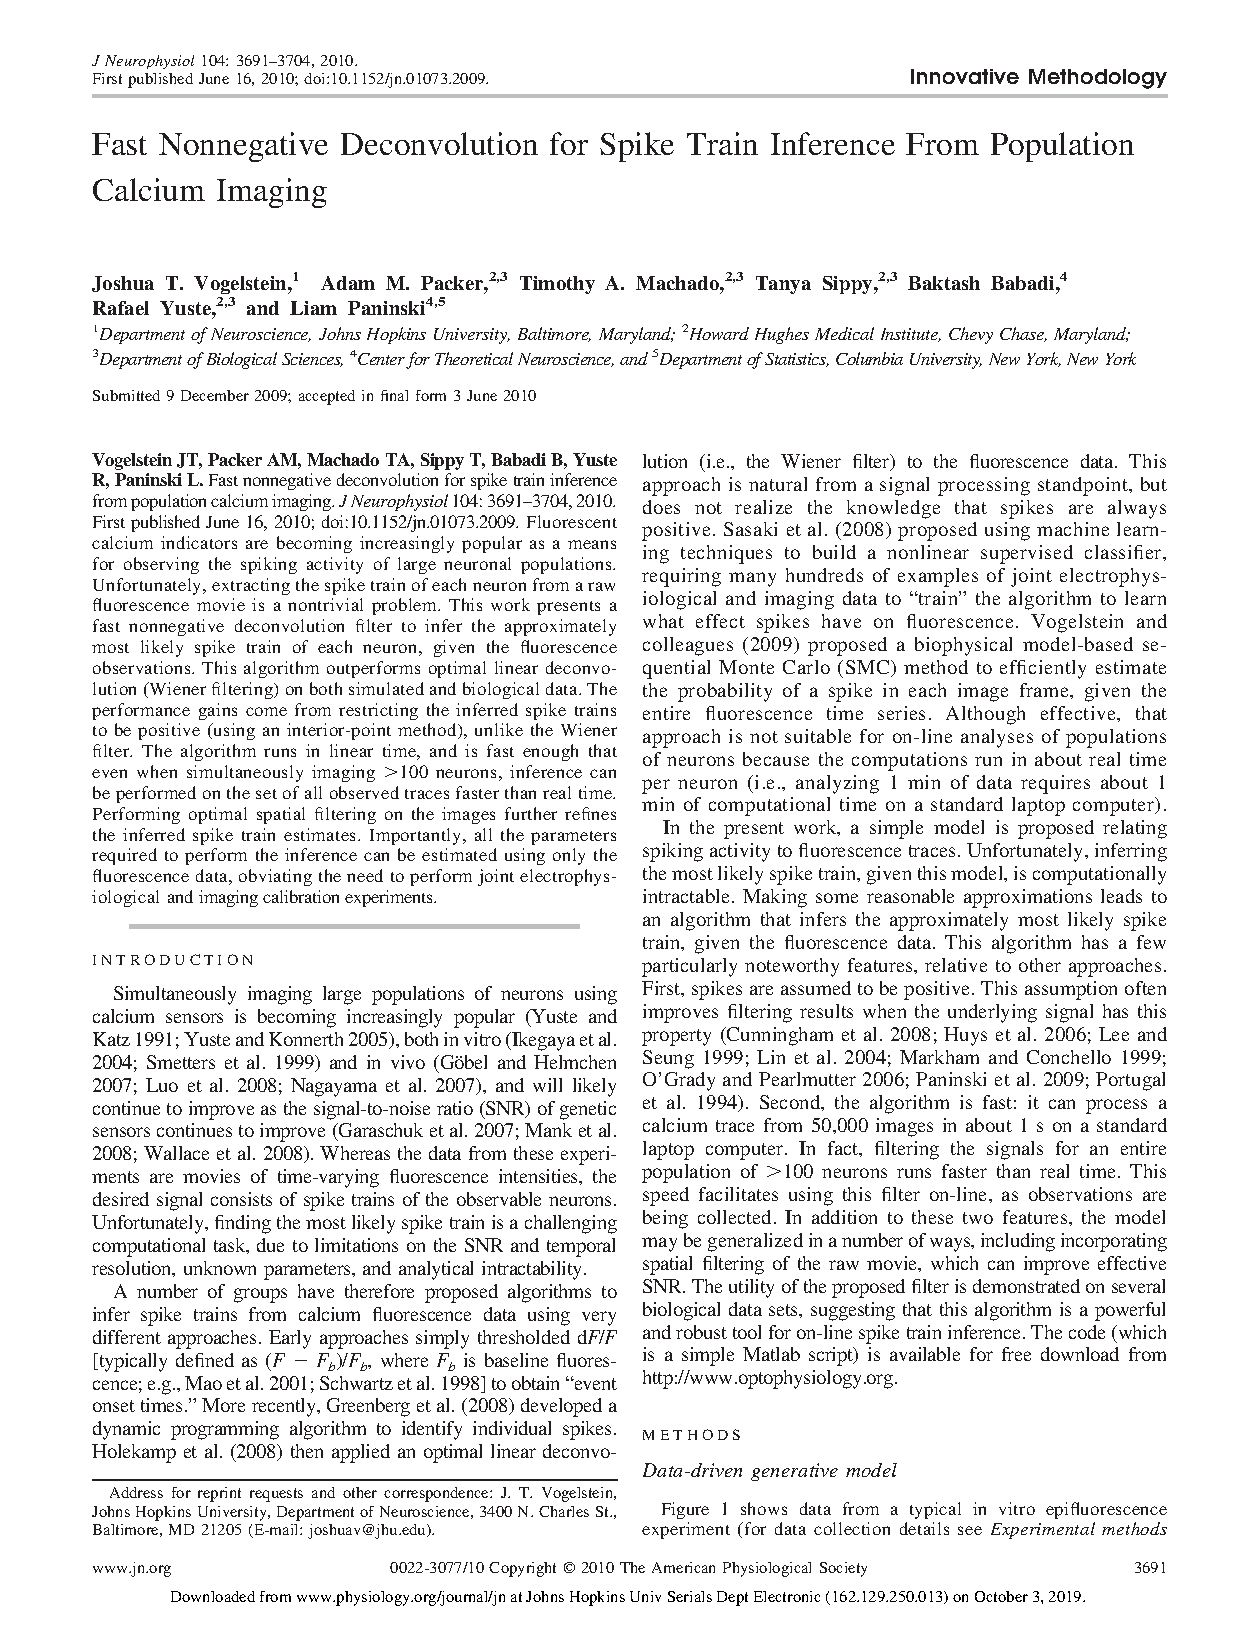
\includepdf[pages=-]{foopsi.pdf}
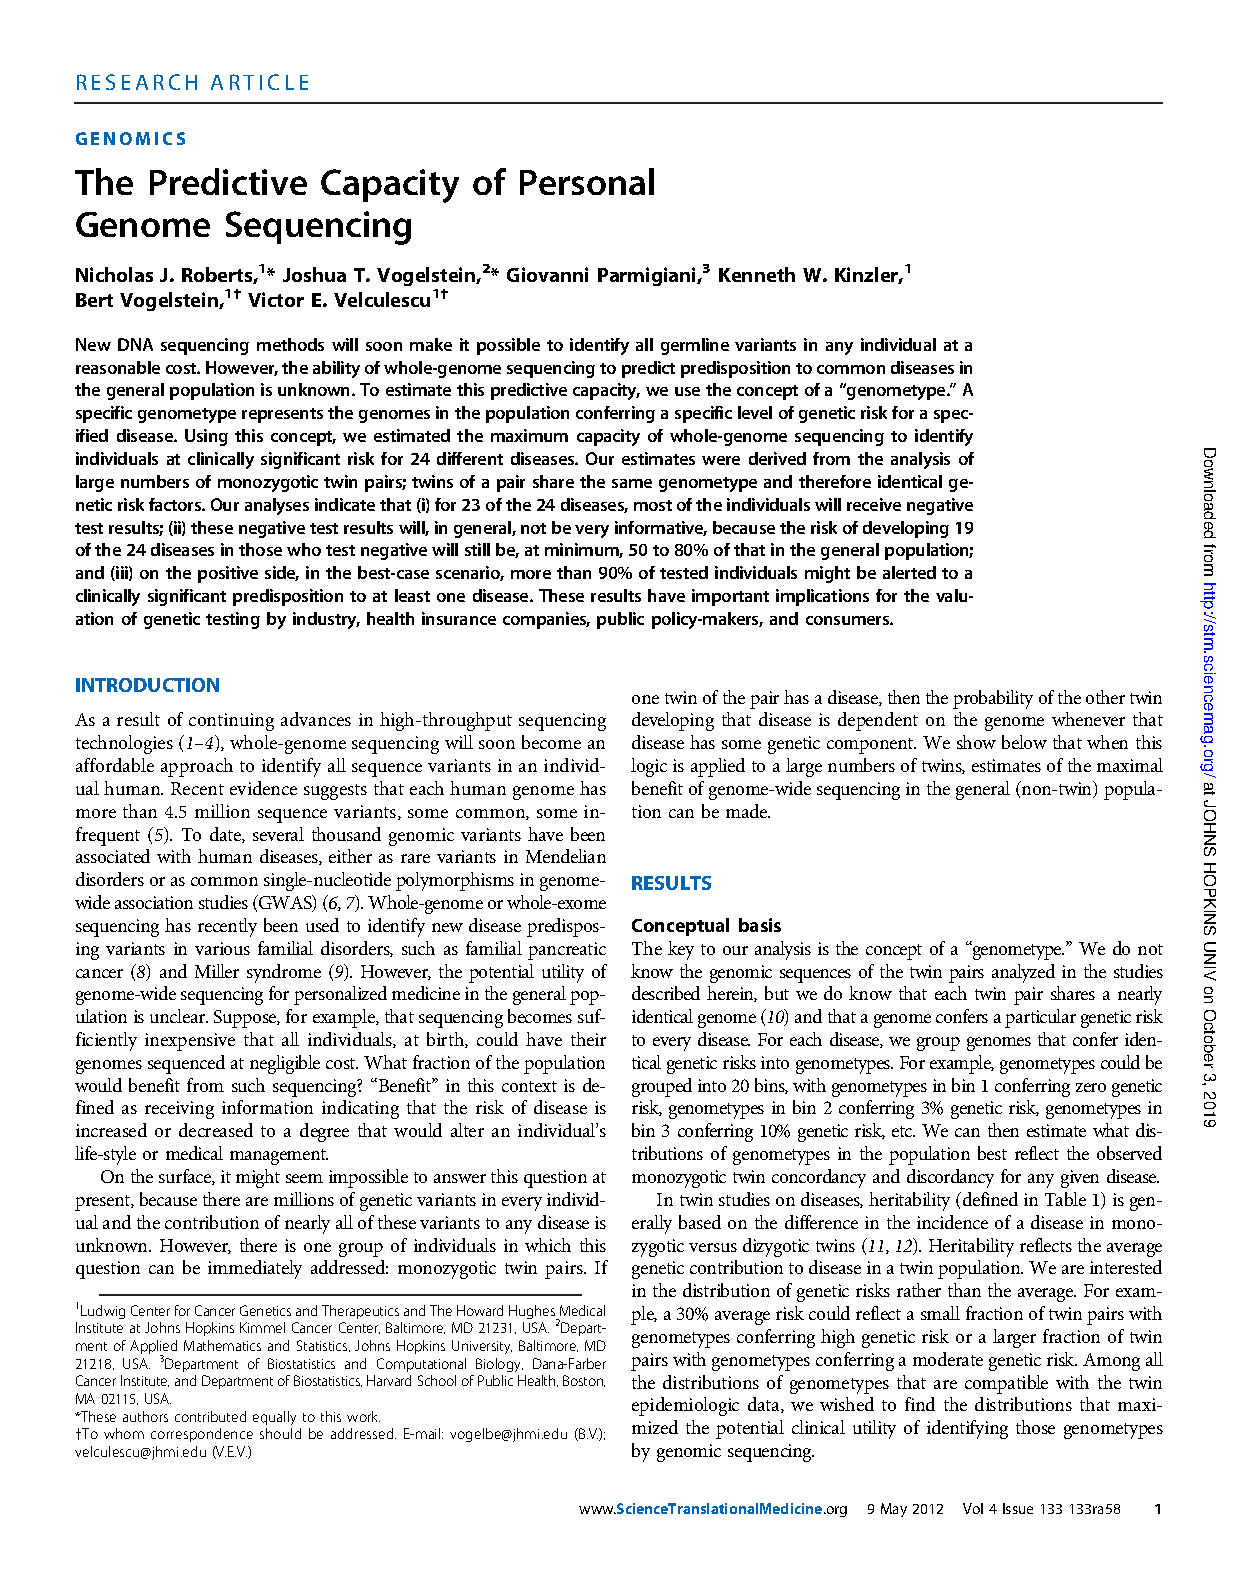
\includepdf[pages=-]{predictive.pdf}
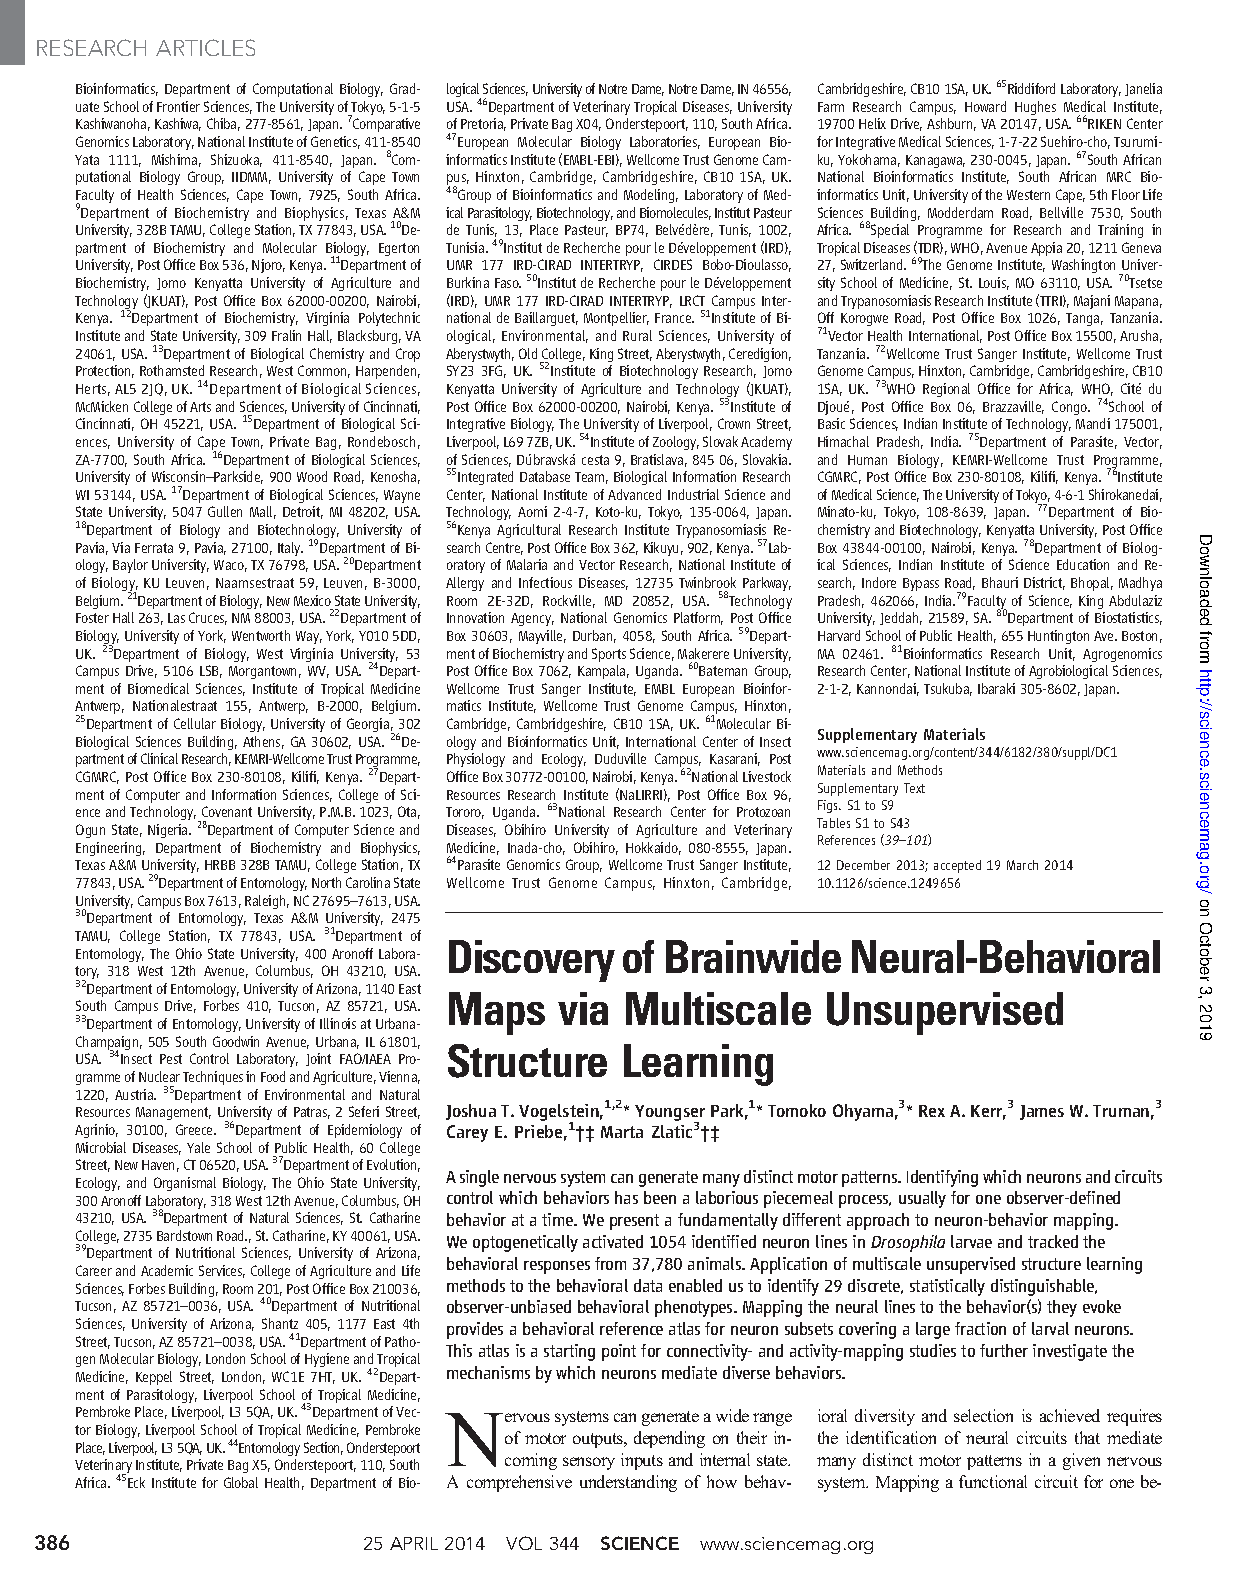
\includepdf[pages=-]{musl.pdf}
\includepdf[pages=-]{ToTheCloud.pdf}


\end{document}
